% !TeX root = ../main.tex

Dato il processo di sviluppo delle applicazioni mobile individuato nel capitolo \ref{ch:ch2} e definiti i principali strumenti che si intende utilizzare nel capitolo \ref{ch:ch3}, si descrive in questo capitolo come è stato automatizzato il processo di sviluppo adottando le moderne tecniche di integrazione continua e rilascio continuo al fine di fornire un modello riutilizzabile ai vari reparti aziendali che si occupano dello sviluppo di applicazioni mobile.\\
Per la progettazione della pipeline è stato utilizzato il progetto base generato tramite il plugin Gradle KMM con lo scopo di mantenere il focus solamente sul processo e non sullo sviluppo del prodotto. Tale progetto fornisce una applicazione essenziale realizzata tramite KMM, comprensiva di modulo condiviso per la logica applicativa e moduli specifici Android e iOS per l'interfaccia utente.\\
Il workflow ideale, e quindi anche la pipeline obiettivo, è composta dai seguenti passi nello stesso ordine in cui sono indicati:
\begin{itemize}
    \item \textit{Pre} - Fase iniziale di preparazione dell'ambiente. In questa fase è necessario configurare tutti gli strumenti necessari alla esecuzione dei passi che seguono fino al termine della pipeline.
    \item \textit{Build} - Compilazione del codice. In questa fase sia il modulo condiviso che le due applicazioni vengono compilate e impacchettate: non è possibile procedere con la fase di testing se anche solo un modulo non compila correttamente.
    \item \textit{Test} - Testing del codice e della interfaccia. Anche in questo caso non è possibile procedere alle fasi successive se i test non passano tutti correttamente.
    \begin{itemize}
        \item \textit{Unit} - Fase di testing della logica applicativa.
        \item \textit{UI} - Fase di testing dell'interfaccia grafica.
    \end{itemize}
    \item \textit{Release} - Fase finale di rilascio delle due applicazioni.
    \begin{itemize}
        \item \textit{Alpha} - Primo rilascio a scopo di testing interno.
        \item \textit{Beta} - Secondo rilascio a scopo di testing esterno, effettuato dopo la validazione interna.
        \item \textit{Prod} - Rilascio finale in produzione, ovvero sui relativi store, che avviene dopo la validazione esterna.
    \end{itemize}
\end{itemize}

\begin{figure}[H]
\centering
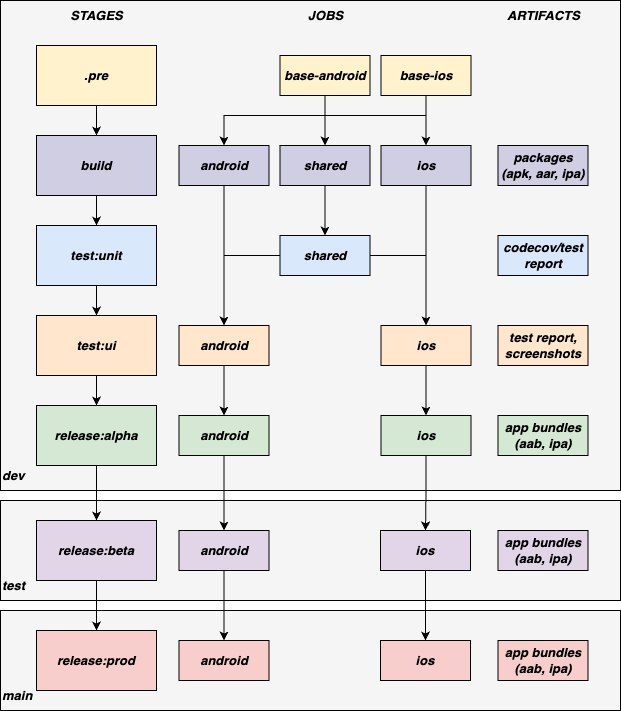
\includegraphics[width=0.8\textwidth]{img/tesi-11-cicd.drawio.png}
\caption{Pipeline obiettivo per la pubblicazione automatica di una applicazione Android e iOS con modulo condiviso}
\end{figure}

\section{Infrastruttura}
L'infrastruttura aziendale a supporto di tutti i processi di sviluppo è di tipo multi-cloud ibrido. E' composta infatti da servizi completamente gestiti da diversi cloud provider, da servizi ospitati sul cloud ma auto-gestiti e da installazioni interne su hardware proprietario. I seguenti rappresentano tutti i componenti infrastrutturali necessari al processo di sviluppo automatizzato progettato per lo sviluppo di applicazioni mobile:
\begin{itemize}
    \item \textit{SonarQube, Nexus Sonatype, GitLab Runner (Linux)} - Servizi disponibili per tutti i team di sviluppo Maggioli e ospitati su Google Cloud.
    \item \textit{GitLab Cloud} - Licenza aziendale per tutti gli sviluppatori Maggioli.
    \item \textit{Cluster Kubernetes, Container Registry} - Servizi disponibili per il solo team di Ricerca e Sviluppo e ospitati su Microsoft Azure.
    \item \textit{Google Play Console, Testflight} - Servizi specifici per lo sviluppo di applicazioni Android e iOS, per i quali sono stati sottoscritti account developer appositi per questo progetto di tesi.
    \item \textit{GitLab Runner (MacOS)} - Servizio interno per l'esecuzione delle pipeline in ambiente Apple, specifico per questo progetto di tesi.
\end{itemize}

\begin{figure}[H]
\centering
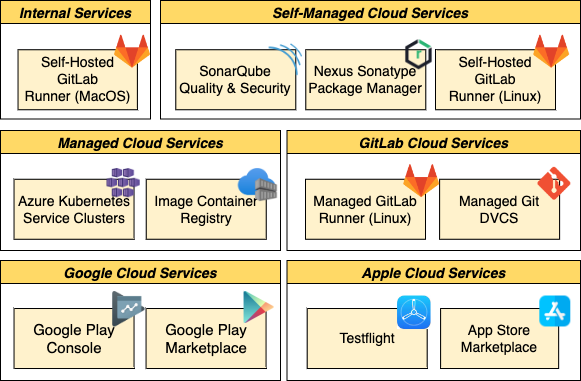
\includegraphics[width=0.8\textwidth]{img/tesi-3-infra.drawio.png}
\caption{Componenti della infrastruttura necessaria a supporto del processo di sviluppo progettato}
\end{figure}

\subsection{MacOS GitLab Runner (Self-Hosted)}
La toolchain di base per lo sviluppo di applicazioni iOS è interamente di proprietà Apple e rende necessario l'utilizzo di una macchina MacOS definendo una serie di vincoli per quanto riguarda sia lo sviluppo locale che l'automazione del processo.

% indicare le varie possibilità (come scritto nelle conclusioni) e dire che è stata scelta l'opzione self-hosted gitlab perchè si voleva avere la possibilità di gestire il runner a 360 gradi (cosa non possibile con quelli managed) in modo da capirne il funzionamento e anche per i costi (molto elevati in termini di euro ad esempio in caso di vm amazon)

\subsubsection{Architettura Runner}
Ogni job di ogni stage definito in una pipeline viene eseguito da un componente software chiamato \textit{runner}. Tramite il modello client-server il runner interroga continuamente il server (ovvero GitLab) per ottenere le informazioni necessarie all'esecuzione dei job. La politica di scheduling dei job fra i vari runner è definita lato server ma può essere pilotata tramite il concetto di \textit{tag}.

\begin{figure}[H]
\centering
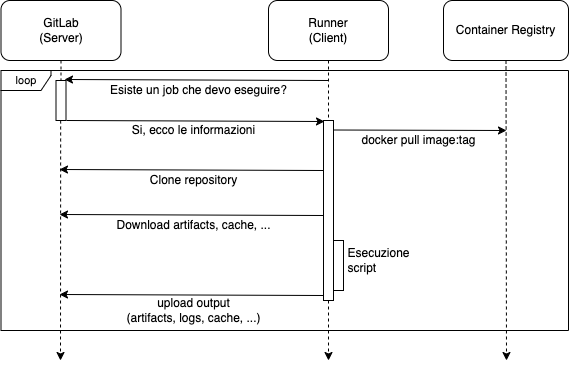
\includegraphics[width=0.8\textwidth]{img/tesi-17-runner.drawio.png}
\caption{Diagramma di sequenza GitLab Runner (Docker Executor)}
\label{fig:archrunner}
\end{figure}

In base a chi lo gestisce, il runner può essere:
\begin{itemize}
    \item \textit{Managed} - Runner gestito da GitLab e fornito in modalità as-a-Service. E' soggetto ad alcune restrizioni di utilizzo che dipendono dal piano di licenza sottoscritto: tipicamente questi limiti coinvolgono il tempo di esecuzione e lo spazio di archiviazione (utilizzo CPU e memoria).
    \item \textit{Self-Hosted} - Runner gestito interamente dall'utente (installazione, configurazione, registrazione, manutenzione, aggiornamento, ...). A differenza dei runner managed, questa modalità non prevede alcun vincolo di utilizzo.
\end{itemize}

Essendo il runner ad iniziare la comunicazione verso il server, uno dei principali vantaggi è quello di poterlo installare anche all'interno di una rete privata senza esporlo pubblicamente. La modalità self-hosted per l'installazione del runner MacOS è stata una scelta obbligata dai vincoli della toolchain Apple ma è comunque preferita sia per l'assenza di vincoli di utilizzo che per l'esecuzione nella rete privata aziendale Maggioli.

\subsubsection{Shell Executor}
L'esecuzione dei job avviene in modo asincrono tramite l'esecuzione di task sottoposti ad un executor. Una entità master si occupa quindi di ottenere i job da far eseguire all'executor, il quale restituisce il risultato una volta terminato. Il grado di concorrenza dell'executor, ovvero il numero di job che possono essere eseguiti in parallelo, è configurabile dalle impostazioni del runner. Le principali tipologie di executor sono\footnote{\url{https://docs.gitlab.com/runner/executors/}}:
\begin{itemize}
    \item \textit{Shell} - Per ogni job viene aperta una shell sulla macchina host in cui è in esecuzione il runner. Tutte le dipendenze necessarie alla esecuzione dei job devono essere installate sulla macchina.
    \item \textit{Container} - L'ambiente di esecuzione dei job è circoscritto all'interno di un container, sia nel caso dell'executor Docker che dell'executor Kubernetes (Pods). Tutte le dipendenze necessarie alla esecuzione dei job devono essere installate all'interno del container utilizzato.
    \item \textit{Virtual Machine} - I job vengono eseguiti all'interno di virtual machine, VirtualBox o Parallels, già preconfigurate.
\end{itemize}

Data la assenza di container basati su sistema operativo MacOS, l'unica opzione accettabile è quella dell'executor di tipo shell attraverso l'installazione\footnote{\url{https://docs.gitlab.com/runner/install/osx.html}} di un runner su una macchina fisica Apple all'interno della rete privata aziendale Maggioli.

\subsubsection{Configurazione}
A prescindere dalla tipologia di executor, per l'utilizzo di un runner GitLab self-hosted è necessario effettuarne installazione, configurazione e avvio. Nel caso di un executor shell è necessario installare il binario\footnote{\url{https://gitlab-runner-downloads.s3.amazonaws.com/latest/binaries/gitlab-runner-darwin-arm64}} mentre nel caso di un executor Docker/Kubernetes è necessario effettuare il deploy del container\footnote{\url{https://hub.docker.com/r/gitlab/gitlab-runner}}. La fase di configurazione del runner varia a seconda del tipo di executor. Per la tipologia di runner scelta per questo progetto di tesi gli aspetti principali configurati sono:
\begin{itemize}
    \item \textit{Registrazione} - Come descritto nella architettura (figura \ref{fig:archrunner}) un runner GitLab interroga continuamente il server per ottenere job da eseguire. E' necessario specificare sia l'indirizzo URL del server GitLab che il gruppo o il progetto per il quale il runner deve eseguire i job. Altri parametri come \textit{locked}, \textit{tag-list} e \textit{run-untagged} sono stati utilizzati per limitare l'accesso del runner al solo repository utilizzato per questo progetto di tesi.
    \begin{listing}[H]
    \inputminted{bash}{code/4-macos-runner-setup}
    \caption{Comandi bash utilizzati per l'installazione e la configurazione di un runner MacOS}
    \end{listing}
    \item \textit{Cache Condivisa} - Permette di condividere uno storage cloud (Google Cloud Storage Buckets in questo caso) per il caching di tutte le dipendenze comuni tra i vari job eseguiti concorrentemente dal runner. L'utilizzo di cache condivisa con un executor shell comporta un vantaggio nell'utilizzo dello spazio disco della macchina in cui è in esecuzione il runner ma non nel tempo di esecuzione delle pipeline, il quale sarebbe molto più ridotto nel caso di cache locale.
\end{itemize}

\begin{listing}[H]
\inputminted{toml}{code/4-macos-runner-config}
\caption{File di configurazione (\textit{config.toml}) generato al momento della registrazione del runner}
\end{listing}

\begin{figure}[H]
\centering
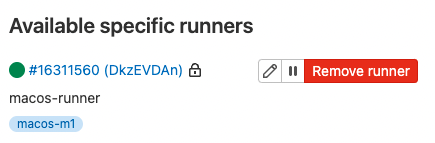
\includegraphics[width=0.6\textwidth]{img/Screenshot 2022-07-07 at 11.40.13.png}
\caption{Screenshot GitLab Web UI: Runner MacOS Self-Hosted correttamente registrato e attivo}
\end{figure}

\section{Modello di Branching}
L'utilizzo di un adeguato flusso di lavoro è fondamentale per definire una efficiente automazione CI/CD. Con branching si intende l'utilizzo di uno o più flussi principali dai quali divergono altri flussi per svolgere determinati lavori per poi convergere al loro termine: in base alle modalità di apertura e chiusura di questi flussi si definiscono diversi modelli di branching.

\begin{figure}[H]
\centering
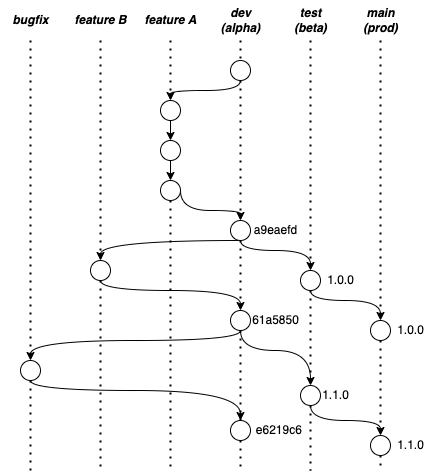
\includegraphics[width=0.6\textwidth]{img/tesi-13-branching.drawio.png}
\caption{Esempio di flusso di sviluppo adottando il modello di branching indicato}
\label{branching}
\end{figure}

Il modello che si intende utilizzare (figura \ref{branching}) è basato sul modello di branching GitFlow\footnote{\url{https://www.atlassian.com/it/git/tutorials/comparing-workflows/gitflow-workflow}} il quale prevede tre branch principali:
\begin{itemize}
    \item \textit{dev} - Flusso principale di sviluppo. Ogni modifica apportata a questo branch corrisponde al rilascio di una nuova versione \textit{alpha}. E' da questo branch che vengono aperti e chiusi nuovi branch, sia per lo sviluppo di nuove funzionalità (\textit{feature}) che per la risoluzione di bug/patch (\textit{fix}).
    \item \textit{test} - Branch modificato solamente tramite merge di modifiche provenienti dal branch \textit{dev} con lo scopo di rilasciare una nuova versione \textit{beta}.
    \item \textit{main} - Branch modificato solamente tramite merge di modifiche provenienti dal branch \textit{test} con lo scopo di rilasciare una nuova versione in produzione (\textit{prod}).
\end{itemize}

Grazie ai meccanismi di automazione a supporto della CI/CD si definiscono specifiche regole di attivazione basate sulle modifiche apportate al codice come ad esempio la modifica di un certo file su un determinato branch.

\section{Continuous Integration}
La pratica di integrare molto frequentemente piccole modifiche al flusso di sviluppo principale è alla base della Continous Integration e permette di diminuire la presenza di problemi rispetto alla integrazione meno frequente di grandi modifiche. Ogni modifica effettuata al codice viene validata automaticamente attraverso l'esecuzione di tutti i passi della pipeline che compongono la fase di integrazione, ovvero compilazione e testing.

\begin{figure}[H]
\centering
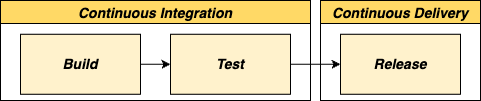
\includegraphics[width=0.7\textwidth]{img/tesi-29-cicd.drawio.png}
\caption{Suddivisione delle fasi di un pipeline in base alle pratiche Continuous Integration/Delivery}
\end{figure}

\subsection{Pre}
Molti dei passi che compongono una pipeline utilizzano tipicamente gli stessi tools e le stesse configurazioni per svolgere task diversi. Un classico esempio è la compilazione del codice e l'esecuzione degli unit test per una applicazione Java: in entrambi i passi viene utilizzata la stessa JDK, lo stesso tool di build automation (Gradle per esempio) e devono essere scaricate le stesse dipendenze del progetto dal repository Maven Central.\\
Utilizzando meccanismi di caching e passaggio di artefatti è possibile eseguire tutti quei task di configurazione una sola volta all'inizio della pipeline risparmiando tempo e risorse in tutte le successive fasi.\\
Nel caso della pipeline progettata per lo sviluppo di applicazioni multiplatform con KMM in questa fase iniziale è necessario eseguire i seguenti task:
\begin{itemize}
    \item Configurazione dell'ambiente per lo sviluppo Kotlin tramite l'installazione del SDK/JDK utilizzando \textit{sdkman}\footnote{\url{https://sdkman.io/}}.
    \item Configurazione dell'ambiente per lo sviluppo Android tramite l'installazione del SDK Android target e dei vari tools necessari utilizzando \textit{sdkmanager}\footnote{\url{https://developer.android.com/studio/command-line/sdkmanager}}.
    \item Configurazione dell'ambiente per lo sviluppo iOS.
    \item Installazione di tutte le dipendenze dei vari moduli con relative tecniche di caching. Tra queste si trova anche il compilatore \textit{Kotlin/Native}\footnote{\url{https://kotlinlang.org/docs/native-improving-compilation-time.html\#general-recommendations}}.
    \item Configurazione delle chiavi per l'autenticazione ai vari servizi cloud forniti da Google e Apple.
\end{itemize}

\subsection{Build}
Tipicamente la fase iniziale della integrazione continua consiste nella verifica della corretta compilazione del codice sorgente. La compilazione rappresenta un vincolo essenziale per tutte le successive fasi e per questo è definita come fase bloccante: in caso di compilazione fallita la pipeline termina senza procedere con le fasi successive.

\begin{listing}[H]
\inputminted{yaml}{code/4-buildjob}
\caption{Pipeline job dedicato compilazione e pacchettizzazione della applicazione Android}
\end{listing}

Nel caso della automazione dello sviluppo di applicazioni mobile per la fase iniziale di build la pratica più diffusa è quella di validare sia la compilazione del codice, ovvero il codice condiviso (Kotlin) e il codice specifico Android (Kotlin)/iOS (Swift), che la pacchettizzazione della applicazione nei formati richiesti dalle piattaforme target (\textit{.apk}\footnote{Android Package} per Android e \textit{.ipa}\footnote{iOS App Store Package} per iOS).

\begin{listing}[H]
\inputminted{ruby}{code/4-buildft}
\caption{Lane Fastlane dedicata alla fase di build tramite l'utilizzo della action Gradle}
\end{listing}

\subsection{Testing}
Dopo aver verificato la corretta compilazione e pacchettizzazione del codice segue la fase di test. Si distinguono due tipologie di testing con lo scopo di validare sia la logica applicativa (\textit{unit testing}) che l'interfaccia grafica (\textit{ui testing}).

\subsubsection{Unit Testing}
Con unit testing si intende l'attività di verifica di certe porzioni (unità) del codice ed è implementato tipicamente utilizzando librerie predisposte per ciascun linguaggio di programmazione. Questa fase di test potrebbe coinvolgere tutti i moduli anche se la business logic è racchiusa solamente nel modulo condiviso perchè in alcune situazioni si fa uso di costrutti specifici della piattaforma target dove è necessario l'utilizzo dell'apposito SDK e runtime. La tipologia di test che necessita dell'esecuzione sul dispositivo, che esso sia fisico o emulato, per sfruttare il framework della piattaforma target è detta \textit{Instrumented Testing}. Una alternativa alla esecuzione dei test sul dispositivo è l'utilizzo di entità \textit{mock} per fornire le stesse funzionalità della piattaforma target.\\
Le librerie utilizzate per la fase di unit testing sono:
\begin{itemize}
    \item \textit{JUnit}\footnote{\url{https://junit.org/junit5/}} (Java/Kotlin) - Framework di unit testing per il linguaggio di programmazione Java.
    \item \textit{XCTest}\footnote{\url{https://developer.apple.com/documentation/xctest}} (Swift/Objective-C) - Framework standard di testing per progetti XCode, tra cui unit testing.
\end{itemize}

\subsubsection{UI Testing}
Analogamente agli unit test, dove si verifica l'integrità della business logic a fronte di una modifica al codice sorgente, negli UI test si verifica l'integrità dell'interfaccia grafica. I moduli per il quale deve essere testata l'interfaccia grafica corrispondono ai moduli delle applicazioni Android e iOS. Le librerie utilizzate per il testing dell'interfaccia grafica delle relative applicazioni sono:
\begin{itemize}
    \item \textit{Espresso}\footnote{\url{https://developer.android.com/training/testing/espresso}} (Android) - Framework standard per ui testing di applicazioni Android.
    \item \textit{XCTest} (iOS) - Framework standard di testing per progetti XCode, tra cui ui testing (XCUI\footnote{\url{https://developer.apple.com/documentation/xctest/user_interface_tests}}).
\end{itemize}
In questa specifica fase del processo tipicamente si realizzano anche degli screenshot delle applicazioni in esecuzione in modo da poterli utilizzare nelle successive fasi di rilascio delle applicazioni. Anche in questo caso sono necessari tool differenti per le due piattaforme, i quali sono compresi nella installazione di Fastlane:
\begin{itemize}
    \item \textit{Screengrab}\footnote{\url{https://docs.fastlane.tools/actions/screengrab/}} (Android) - Richiede la definizione di appositi test utilizzando \textit{Espresso} per navigare nella applicazione in esecuzione e della libreria \textit{tools.fastlane:screengrab} per la cattura delle schermate.
    \item \textit{Snapshot}\footnote{\url{https://docs.fastlane.tools/actions/snapshot/}} (iOS) - Tramite il comando di inizializzazione fornito dal tool viene generato il codice Swift (\textit{SnapshotHelper.swift}) di supporto alla cattura degli screenshot per la applicazione iOS. Anche in questo caso è necessario utilizzare l'apposito framework di test per la navigazione della applicazione in esecuzione.
\end{itemize}

\begin{listing}[H]
\inputminted{swift}{code/4-ios-screenshot}
\caption{Codice Swift d'esempio per la cattura degli screenshot della applicazione iOS}
\end{listing}

Per entrambe le piattaforme sia i test che la cattura delle schermate necessitano l'emulazione headless, ovvero con l'interfaccia utente disattivata, dei dispositivi target. Ogni dispositivo emulato richiede un insieme di risorse tale da non permettere l'esecuzione dei test sull'interfaccia in modo parallelo. Per gestire queste situazioni GitLab fornisce un apposito costrutto, chiamato \textit{resource\_group}: ogni job in cui è dichiarato lo stesso resource\_group viene eseguito in modo mutualmente esclusivo.

\begin{listing}[H]
\inputminted{yaml}{code/4-screenshot-ui-android}
\caption{Pipeline job dedicato al testing della interfaccia grafica e alla cattura delle schermate (Android)}
\end{listing}

\section{Continuous Delivery}
La pratica Continuous Delivery applica gli stessi concetti della Continuous Integration alla fase di rilascio: prevede infatti che il rilascio di una nuova versione avvenga in modo automatico e molto frequente con piccole modifiche apportate al codice.\\
Nel caso dello sviluppo di applicazioni multiplatform con Kotlin KMM bisogna considerare che le due applicazioni potrebbero essere rilasciate singolarmente, avere versioni differenti e che i possibili scenari in cui si effettua un rilascio sono:
\begin{itemize}
    \item Modifica al codice condiviso (rilascio di una nuova versione per entrambe le piattaforme).
    \item Modifica alla interfaccia utente (rilascio di una nuova versione per soltanto una piattaforma oppure entrambe).
\end{itemize}

\subsection{Google Play Console}
A differenza delle applicazioni iOS, le quali richiedono due strumenti separati per la pubblicazione e per il testing, le applicazioni Android vengono gestite interamente da una unica piattaforma chiamata Google Play Console. Tramite il concetto di \textit{promozione} una specifica versione di applicazione viene infatti promossa da \textit{alpha} a \textit{beta} o da \textit{beta} a \textit{produzione}.

\begin{listing}[H]
\inputminted{ruby}{code/4-gpc-promote}
\caption{Esempio di Lane Fastlane per la promozione di un rilascio Android da \textit{alpha} a \textit{beta}}
\end{listing}

Per integrare correttamente nel processo di sviluppo automatizzato le fasi di pubblicazione e testing da parte degli utenti è necessario svolgere le seguenti azioni:
\begin{itemize}
    \item Creazione account Google Developer.
    \item Creazione scheletro iniziale della app dalla piattaforma Google Play Console.
    \begin{itemize}
        \item Classificazione PEGI\footnote{\url{https://pegi.info/it}}.
        \item Creazione mailing-list alpha e beta tester. Tali tester per poter scaricare la applicazione tramite il link condiviso, il quale reindirizza alla pagina corretta di download sul Play Store, devono aver abilitato l'opzione "Internal App Sharing" dalle impostazioni della applicazione Play Store sul proprio dispositivo Android.
        \item Configurazione monetizzazione, pubblicità/annunci, ... .
    \end{itemize}
    \item Creazione Service Account, utile a identificare/autenticare/autorizzare la applicazione creata sui servizi Google (in questa fase è necessario intervenire anche sulla piattaforma Google Cloud Platform).
    \begin{itemize}
        \item Test Connessione Fastlane-Play Store.
        \item Setup service\_account\_key.json nei segreti GitLab per essere utilizzata dinamicamente nella pipeline senza essere versionata nei sorgenti.
    \end{itemize}
    \item Creazione chiavi, in formato \textit{Java KeyStore} (jks) per firmare l'applicazione da pubblicare.
    \begin{itemize}
        \item Setup chiave jks nei segreti GitLab per essere utilizzata dinamicamente nella pipeline senza essere versionata nei sorgenti. Dato che al momento della scrittura di questa tesi GitLab non fornisce la possibilità di inserire file binari tra i segreti è stato necessario codificare in formato esadecimale la chiave generata in modo da poterla salvare come variabile testuale e decodificarla durante l'esecuzione della pipeline\cite{gitlabciandroid}.
        \begin{listing}[H]
        \inputminted{bash}{code/4-jks}
        \caption{Creazione, codifica e decodifica della chiave JKS}
        \end{listing}
    \end{itemize}
    \item Upload manuale della prima release della applicazione. Da Agosto 2021\footnote{\url{https://developer.android.com/guide/app-bundle}} il formato di pubblicazione delle applicazioni Android \textit{aab} (Android Application Bundle) ha sostituito il formato \textit{apk}. Gli apk scaricabili e installabili sui dispositivi vengono creati automaticamente dal Play Store a partire dal aab caricato.
\end{itemize}

\subsection{TestFlight}
La configurazione degli strumenti utili al rilascio automatizzato di applicazioni iOS è molto simile a quello sopra descritto per l'ecosistema Android: 
\begin{itemize}
    \item Creazione account Apple Developer.
    \item Creazione certificato del tipo \textit{iOS Distribution} (Certificate Signing Request\footnote{\url{https://help.apple.com/developer-account/\#/devbfa00fef7}}) tramite il portale App Store Connect.
    \item Creazione provisioning profile del tipo \textit{App Store} collegato al certificato appena creato e successiva installazione tramite Xcode.
    \item Assegnamento dei permessi a \textit{codesign} (il tool Apple utilizzato per firmare l'applicazione) in modo che possa accedere ai certificati autenticandosi al gestore \textit{Keychain Access}.
    \item Creazione api key per autenticazione ai servizi App Store Connect, come richiesto da Fastlane\footnote{\url{https://docs.fastlane.tools/app-store-connect-api/\#using-fastlane-api-key-json-file}}.
    \item Creazione App-Specific Password dal proprio profilo Apple ID per autenticazione tramite \textit{transporter}\footnote{\url{https://help.apple.com/itc/transporteruserguide/en.lproj/static.html\#itc16ef2f321}}, ovvero il tool utilizzato da Fastlane per effettuare l'upload della applicazione. 
    \begin{itemize}
        \item La password generata può essere passata a Fastlane solamente tramite variabile d'ambiente, appositamente settata nei segreti GitLab.
    \end{itemize}
    \item Creazione scheletro iniziale della app dalla piattaforma App Store Connect.
    \begin{itemize}
        \item Creazione mailing-list alpha e beta tester. Per poter scaricare la applicazione tramite link condiviso i tester devono aver accettato l'invito di partecipazione e installato l'applicazione Testflight.
        \item Configurazione monetizzazione, pubblicità/annunci, ... .
    \end{itemize}
    \item Configurazione compliance encryption nel file \textit{Info.plist}\footnote{\url{https://help.apple.com/app-store-connect/\#/dev88f5c7bf9}}, necessario per le policy Apple di pubblicazione app e quindi non doverlo configurare manualmente tramite App Store Connect ad ogni release.
\end{itemize}

\subsection{Alpha/Beta Release}
Sia per il rilascio sul Play Store che per quello su Testflight sono stati definiti, tramite gli appositi portali, dei gruppi che identificano l'insieme dei tester interni. Nel caso di Android è possibile pubblicare una release in versione alpha indicando la tipologia di rilascio, chiamata \textit{track}, con il valore "alpha". Per poter successivamente rilasciare la stessa versione in beta è necessario effettuare una promozione sulla relativa track. Nel caso iOS, invece, non è presente il concetto di track: la distinzione tra le tipologie di rilascio viene fatta direttamente tramite i gruppi di tester definiti in Testflight, nello specifico il gruppo "\textit{Internal Tester}" e il gruppo "\textit{External Tester}".

\begin{figure}[H]
\centering
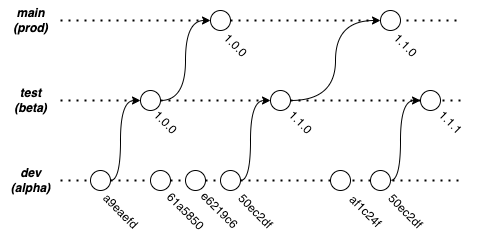
\includegraphics[width=0.8\textwidth]{img/tesi-18-release-flow.drawio.png}
\caption{Esempio di workflow: fasi di release alpha-beta-prod}
\end{figure}

\begin{listing}[H]
\inputminted{yaml}{code/4-ios-alpha}
\caption{Pipeline job dedicato al rilascio in versione alpha della applicazione iOS}
\end{listing}

Per poter informare in modo automatico i tester dell'avvenuto rilascio di una nuova versione è stata scelta, tra le varie integrazioni possibili, la action \textit{slack} fornita da Fastlane perchè Slack\footnote{\url{https://slack.com/intl/it-it/}} viene già utilizzato in Maggioli come software di collaborazione aziendale per la messaggistica istantanea tra i membri dei team. E' necessario prima di tutto creare un canale con tutti i tester e aggiungere un webhook, il cui compito è quello di esporre un endpoint per l'invio di messaggi tramite chiamate HTTP.

\begin{figure}[H]
\centering
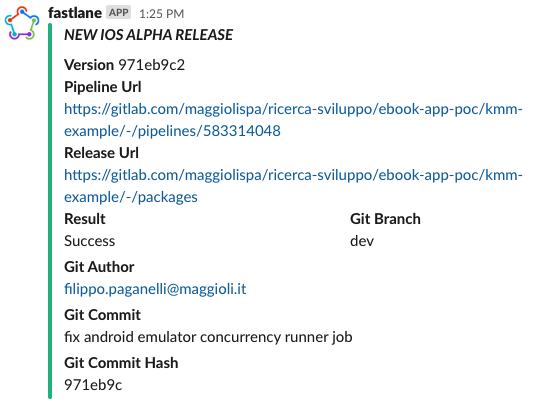
\includegraphics[width=0.7\textwidth]{img/Screenshot 2022-07-08 at 17.48.40.png}
\caption{Screenshot canale Slack: notifica di rilascio applicazione iOS alpha}
\end{figure}

\section{Continuous Inspection}
Tipicamente vengono definiti a livello aziendale degli standard di qualità e di sicurezza che devono essere rispettati da ogni team di sviluppo per qualsiasi prodotto software. La definizione di linee guida sullo stile di programmazione è un classico esempio di standard di qualità. La pratica di analizzare automaticamente e molto frequentemente il codice al fine di validare il rispetto degli standard di qualità e sicurezza è chiamata Continuous Inspection.
L'obiettivo è quello di ottenere un feedback sia sullo stato del codice e del processo che sulla presenza di problemi di sicurezza al fine di pianificare interventi risolutivi. Per esempio la stima di un elevato debito tecnico accumulato segnala che gli sviluppatori non stanno producendo software di qualità.\\
In questa sezione si descrivono le tecniche di analisi adottate e come queste sono state integrate nel processo di sviluppo sia per il codice sviluppato che per le dipendenze del sistema. Rispettivamente le due tecniche sono:
\begin{itemize}
    \item \textit{Static Application Security Testing} (SAST) - Analisi white-box della applicazione al fine di individuare vulnerabilità, code smell e bug.
    \item \textit{Software Composition Analysis} (SCA) - Analisi delle dipendenze di progetto con lo scopo di individuare vulnerabilità pubbliche (CVE)\footnote{Common Vulnerability and Exposure} associate ad esse.
\end{itemize}

\begin{figure}[H]
\centering
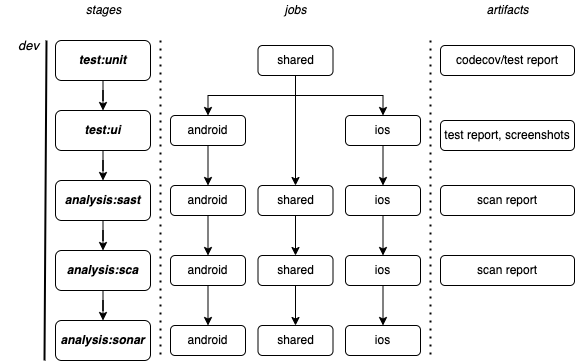
\includegraphics[width=0.8\textwidth]{img/tesi-16-cicd-scheduled.drawio.png}
\caption{Struttura della pipeline schedulata per l'analisi statica del codice}
\end{figure}

In entrambe le tipologie di analisi è fondamentale ottenere come risultato un report della scansione, in grado di descrivere in modo dettagliato eventuali "findings" trovati, ovvero l'insieme delle entità individuate dalla analisi. I report vengono prodotti tipicamente sia in formati human-readable (es. pagina HTML) che machine-readable (es. JSON, XML, ...) per poter essere utilizzati da applicazioni terze come ad esempio sistemi per centralizzare la consultazione di report eterogenei (\textit{Vulnerability Management System}). Nel contesto aziendale Maggioli questi servizi sono messi a disposizione di tutti i team di sviluppo e mantenuti dalle figure responsabili della sicurezza informatica. Nello specifico i servizi aziendali disponibili sono:
\begin{itemize}
    \item \textit{SonarQube}\footnote{\url{https://github.com/SonarSource/sonarqube}} - Piattaforma open-source per effettuare analisi statica del codice.
    \item \textit{Dependency Track}\footnote{\url{https://github.com/DependencyTrack}} - Piattaforma open-source per effettuare l'analisi delle dipendenze (SBOM\footnote{Software Bill Of Material - \url{https://owasp.org/www-community/Component_Analysis\#software-bill-of-materials-sbom}}).
    \item \textit{DefectDojo}\footnote{\url{https://github.com/DefectDojo}} - Piattaforma open-source per la gestione centralizzata delle vulnerabilità tramite l'aggregazione di report proveniente da sorgenti eterogenee.
\end{itemize}

\begin{figure}[H]
\centering
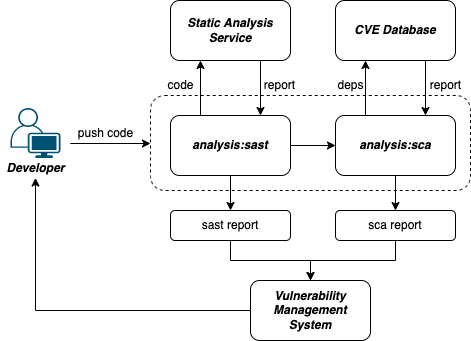
\includegraphics[width=0.8\textwidth]{img/tesi-12-sastsca.drawio.png}
\caption{Esempio tipico di integrazione della analisi statica e delle dipendenze nel processo di sviluppo automatizzato}
\end{figure}

\subsection{Composizione Software}
Con composizione software si intende l'insieme di codice sviluppato da terze parti che viene incluso all'interno della applicazione, tipicamente sotto forma di import di librerie, dette dipendenze. Queste dipendenze includono a loro volta altre dipendenze e potrebbero introdurre vulnerabilità nella applicazione che le utilizza. Per questo motivo è necessario analizzare le dipendenze al fine di individuare le vulnerabilità che esse introducono per essere tempestivi nel loro aggiornamento non appena vengono rilasciate delle patch di sicurezza. Il tool adottato per effettuare questa tipologia di analisi è \textit{DependencyCheck}\footnote{\url{https://github.com/jeremylong/DependencyCheck}}, un tool open-source rilasciato e mantenuto da OWASP disponbile come plugin Gradle, binario eseguibile e immagine Docker.

\begin{listing}[H]
\inputminted{yaml}{code/4-depcheckjob}
\caption{Pipeline job dedicato alla analisi delle dipendenze della applicazione Android tramite l'utilizzo del tool OWASP DependencyCheck}
\end{listing}

\subsection{Analisi Statica}
La fase di analisi statica viene eseguita per il codice condiviso e per il codice specifico considerando i tre moduli separati come moduli indipendenti. I tool individuati e integrati nella fase di analisi statica del codice sono i seguenti:
\begin{itemize}
    \item \textit{Android Lint} (android, condiviso) - Tool per l'analisi statica di applicazioni Android, disponibile come binario eseguibile e plugin Gradle (a partire dalla versione 16 ADT\footnote{Android Development Tools}).
    \item \textit{Detekt} (android, condiviso) - Tool per l' analisi statica del codice, specifico per il linguaggio di programmazione Kotlin, disponibile come binario eseguibile e plugin Gradle.
    \item \textit{SwiftLint} (ios) - Tool per l'analisi statica del codice, specifico per il linguaggio di programmazione Swift, disponibile come binario eseguibile e CocoaPods.
    \item \textit{SonarQube} (android, condiviso, ios) - Client tool per l'interazione con il server SonarQube, disponibile come binario eseguibile e plugin Gradle.
\end{itemize}

\begin{listing}[H]
\inputminted{yaml}{code/4-sastjob}
\caption{Pipeline job dedicato alla analisi statica del codice specifico Android}
\end{listing}

\begin{listing}[H]
\inputminted{ruby}{code/4-sastfastlane}
\caption{Lane Fastlane dedicata alla analisi statica del codice specifico Android}
\end{listing}

Data la funzionalità di gestione delle vulnerabilità fornita dallo stesso SonarQube e la possibilità di integrare tutte le tipologie di report prodotte sia nella fase di analisi delle dipendenze che nella fase di analisi statica del codice, si è deciso di non introdurre nel sistema l'utilizzo dei servizi forniti dalla installazione aziendale di DefectDojo.\\
Per le fasi di analisi i tool utilizzati hanno bisogno soltanto dei sorgenti e dei file di configurazione comportando diversi vantaggi come il fatto di non dover compilare nessun file e di non dover scaricare nessun sdk. Per questi motivi, dove possibile, è stata utilizzata l'immagine Docker del relativo tool come immagine base per il job della pipeline.\\
Il client SonarQube utilizzato è stato dunque configurato agendo sui file degli specifici moduli (\textit{sonar-project.properties}) per poter raccogliere i report prodotti nelle altre fasi di analisi :
\begin{listing}[H]
\inputminted{kotlin}{code/4-sonarplugin}
\caption{Configurazione client SonarQube per il modulo condiviso (Shared)}
\end{listing}
\begin{figure}[H]
\centering
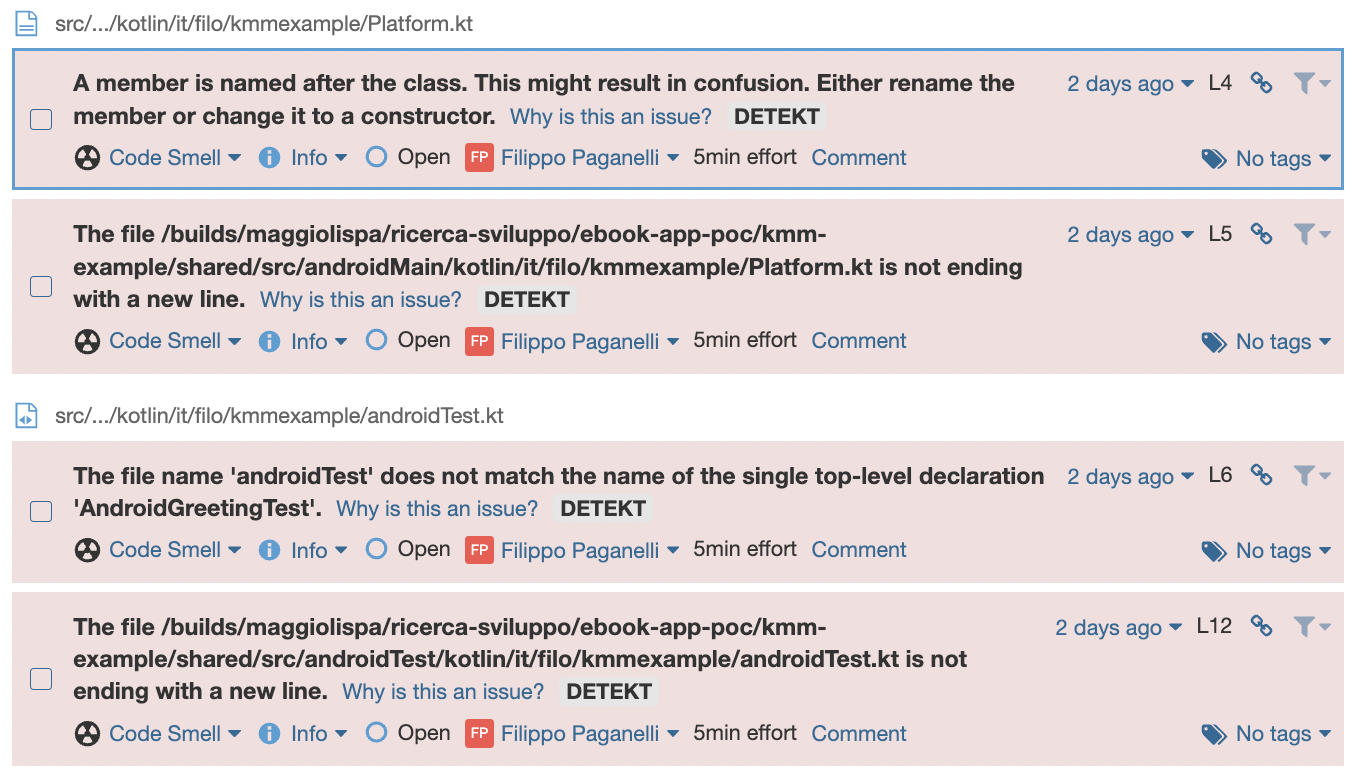
\includegraphics[width=1\textwidth]{img/Screenshot 2022-06-19 at 15.33.37.png}
\caption{Screenshot SonarQube Web UI - Esempio analisi modulo condiviso}
\end{figure}
\begin{figure}[H]
\centering
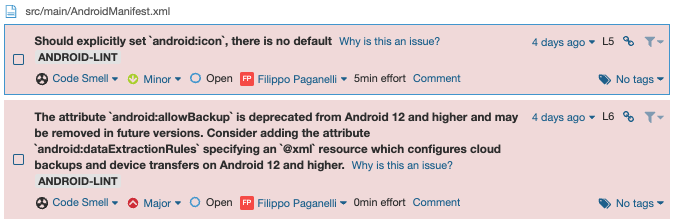
\includegraphics[width=1\textwidth]{img/Screenshot 2022-06-21 at 09.58.58.png}
\caption{Screenshot SonarQube Web UI - Esempio analisi modulo android}
\end{figure}

\subsection{Schedulazione Job}
Le fasi di analisi del codice possono essere introdotte nel processo di sviluppo distinguendo due modalità di esecuzione:
\begin{itemize}
    \item \textit{Sincrona} - L'analisi del codice viene eseguita ad ogni commit su uno specifico branch (in questo caso \textit{dev}). Il vantaggio consiste nella ricezione di un feedback più rapido sulla modifica apportata al codice mentre lo svantaggio è dato da un incremento considerevole nel tempo di esecuzione di ogni pipeline.
    \begin{figure}[H]
    \centering
    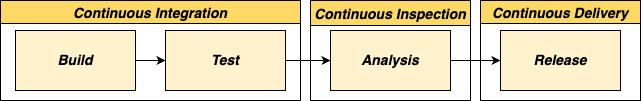
\includegraphics[width=0.7\textwidth]{img/tesi-2-30.cicdci.drawio.png}
    \caption{Approcio sincrono per l'esecuzione della fase di analisi}
    \end{figure}
    \item \textit{Asincrona} - Tramite la schedulazione delle fasi di analisi in un momento diverso da quello in cui viene apportata la modifica al codice è possibile sia ridurre i tempi di esecuzione delle pipeline che ottenere un feedback cumulativo sull'insieme delle modifiche apportate tra due esecuzioni delle pipeline di analisi del codice. Ad esempio, schedulando alla mezzanotte di ogni giorno l'esecuzione delle fasi di analisi, è possibile accedere al portale SonarQube all'inizio della giornata lavorativa successiva e pianificare gli interventi di risoluzione degli eventuali bug introdotti nella giornata precedente.
    \begin{figure}[H]
    \centering
    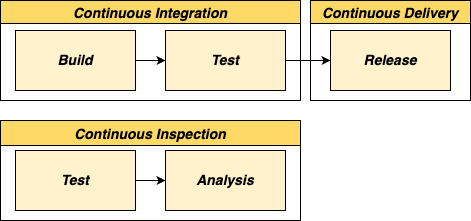
\includegraphics[width=0.59\textwidth]{img/tesi-2-31-cicdci2.drawio.png}
    \caption{Approccio asincrono per l'esecuzione della fase di analisi}
    \end{figure}
\end{itemize}
La modalità di esecuzione scelta per la fase di Continuous Inspection è quella asincrona per le motivazioni sopra indicate, le quali sono vantaggi preferiti dalla maggior parte dei team di sviluppo in Maggioli.

\section{Templating}
L'obiettivo di questo progetto di tesi consiste nella progettazione di una pipeline di CI/CD tale da poter essere riutilizzata dai vari team in azienda che si occupano dello sviluppo di applicazioni mobile. I principali strumenti forniti dalla piattaforma GitLab a supporto del riuso delle pipeline sono:
\begin{itemize}
    \item \textit{Template} - I file YAML che definiscono una pipeline o sottoparte di essa, possono risiedere in un repository diverso da quello in cui si trova il progetto che la utilizza. In questo modo si definisce una sola volta il flusso base per poterlo successivamente includere e/o estendere negli specifici progetti che necessitano il suo utilizzo.
    \item \textit{Include} - Definiti i template è necessario includerli all'interno del file \textit{.gitlab-ci.yml} nella root dello specifico progetto.
    \item \textit{Extend} - Definendo lo script del job padre in modo parametrico è possibile pilotarne il comportamento tramite la definizione di variabili d'ambiente nel job figlio. Questa funzionalità è una alternativa alle \textit{anchors} fornite nativamente da YAML ma più flessibile e leggibile.
    \item \textit{Hidden Jobs} - I job definiti con un punto all'inizio del nome non vengono considerati dal linter GitLab e quindi esclusi dalla esecuzione tramite il runner. Definendo job "nascosti" è possibile definire tutti quegli aspetti comuni e parametrizzati da estendere con altri job.
\end{itemize}

\begin{listing}[H]
\inputminted{yaml}{code/4-templating2}
\caption{Hidden Job base parametrico per i job iOS (\textit{kmm-templates/kmm-base.yml})}
\end{listing}

I seguenti template realizzati sono organizzati in un repository separato, raggruppati logicamente secondo gli stage che compongono l'intera pipeline oltre ad un template base, utilizzato da tutti gli altri template:
\begin{itemize}
    \item \textit{kmm-base} - Definisce tutte le configurazioni di base della pipeline come ad esempio gli stage, variabili d'ambiente globali, job di pre-configurazione, ... .
    \item \textit{kmm-build} - Definisce i job relativi alla fase di compilazione e packaging.
    \item \textit{kmm-test} - Definisce i job per le fasi di unit testing e ui testing.
    \item \textit{kmm-analysis} - Definisce i job per le fasi di analisi statica del codice, analisi delle dipendenze e integrazione con SonarQube.
    \item \textit{kmm-release} - Definisce i job utili al rilascio delle applicazioni sia alpha che beta.
\end{itemize}

\begin{listing}[H]
\inputminted{yaml}{code/4-templating}
\caption{Esempio d'uso dei template GitLab: import da repository remoto}
\end{listing}

I template progettati rimandano all'utilizzatore la definizione delle politiche di attivazione e delle dipendenze in modo da consentirne l'utilizzo in un flusso di lavoro diverso da quello progettato anche in casi di sviluppo con tecnologie differenti.
